\chapter{Entity Relationship Diagram (ERD)}
\label{ch:erd}

\section{Database Overview}
\label{sec:erd-overview}

The \projectname{} database consists of 24 core tables organized into logical domains: User Management, Paper Management, Collaboration, AI Features, Billing, and Admin. The schema is designed for scalability, data integrity, and query performance.

\begin{infobox}[Database Technology]
\begin{itemize}
    \item \textbf{DBMS:} PostgreSQL 15+ with Prisma ORM
    \item \textbf{Hosting:} Railway (Production) / Local (Development)
    \item \textbf{Schema Management:} Prisma Migrate
    \item \textbf{Total Tables:} 24 core entities
    \item \textbf{Indexes:} 8 composite indexes for performance
    \item \textbf{Relationships:} 35+ foreign key constraints
\end{itemize}
\end{infobox}

% ============================================
% ERD DIAGRAM
% ============================================
\section{Complete ERD}
\label{sec:erd-diagram}

\begin{figure}[H]
\centering
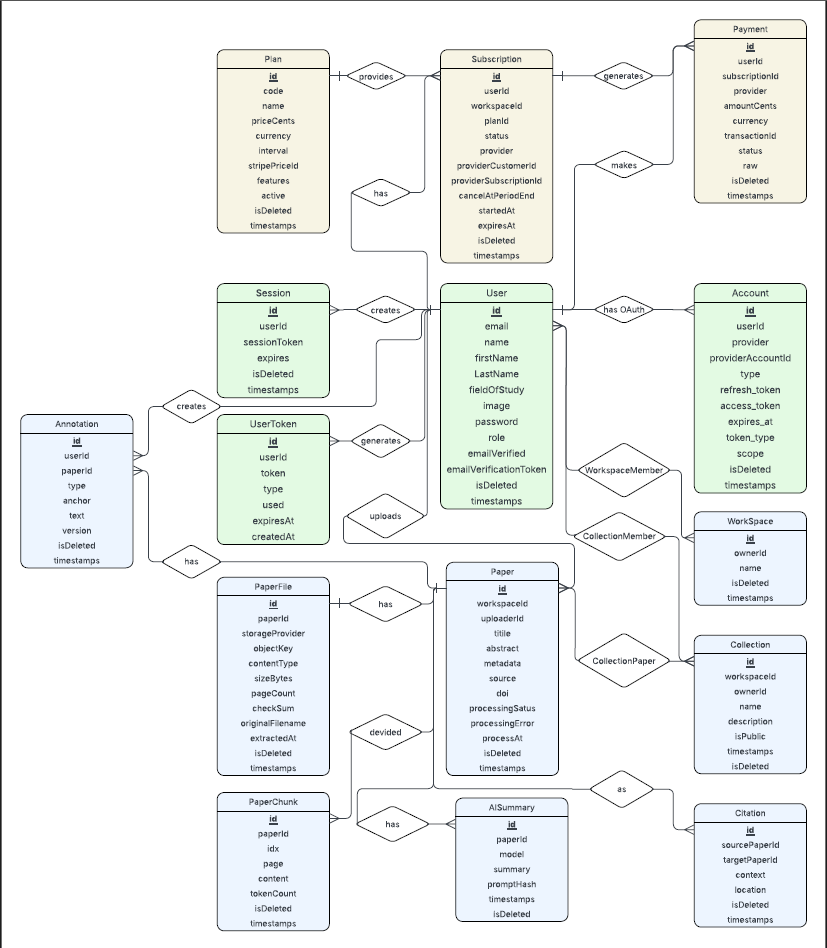
\includegraphics[width=0.95\textwidth]{images/diagrams/ERD.png}
\caption{ScholarFlow Complete Entity Relationship Diagram}
\label{fig:erd-complete}
\end{figure}

\noindent For an interactive version, visit: \url{https://lucid.app/lucidchart/76e3f9ec-0891-48af-aeed-1a6f9dbd641c}

% ============================================
% DOMAIN BREAKDOWN
% ============================================
\section{Domain Organization}
\label{sec:erd-domains}

\subsection{User Management Domain}

\begin{table}[H]
\centering
\caption{User Management Entities}
\label{tab:erd-user-domain}
\begin{tabular}{@{}llp{6cm}@{}}
\toprule
\textbf{Table} & \textbf{Purpose} & \textbf{Key Relationships} \\
\midrule
User & Core user account & Papers, Workspaces, Subscriptions \\
Account & OAuth provider accounts & User (many-to-one) \\
Session & JWT session tracking & User (many-to-one) \\
VerificationToken & Email verification & User (many-to-one) \\
\bottomrule
\end{tabular}
\end{table}

\subsection{Paper Management Domain}

\begin{table}[H]
\centering
\caption{Paper Management Entities}
\label{tab:erd-paper-domain}
\begin{tabular}{@{}llp{6cm}@{}}
\toprule
\textbf{Table} & \textbf{Purpose} & \textbf{Key Relationships} \\
\midrule
Paper & Research paper metadata & User, Workspace, Collections \\
Collection & Paper organization groups & Workspace, Papers, Permissions \\
CollectionPermission & Access control & Collection, User \\
Tag & Paper categorization & Papers (many-to-many) \\
\bottomrule
\end{tabular}
\end{table}

\subsection{Collaboration Domain}

\begin{table}[H]
\centering
\caption{Collaboration Entities}
\label{tab:erd-collaboration-domain}
\begin{tabular}{@{}llp{6cm}@{}}
\toprule
\textbf{Table} & \textbf{Purpose} & \textbf{Key Relationships} \\
\midrule
Workspace & Team collaboration space & User, Papers, Collections \\
WorkspaceMember & Team membership & Workspace, User \\
WorkspaceInvitation & Member invitations & Workspace, User \\
\bottomrule
\end{tabular}
\end{table}

\subsection{AI Features Domain}

\begin{table}[H]
\centering
\caption{AI Features Entities}
\label{tab:erd-ai-domain}
\begin{tabular}{@{}llp{6cm}@{}}
\toprule
\textbf{Table} & \textbf{Purpose} & \textbf{Key Relationships} \\
\midrule
AISummary & AI-generated summaries & Paper (one-to-one) \\
AIChatHistory & Chat conversation logs & Paper, User \\
\bottomrule
\end{tabular}
\end{table}

\subsection{Billing Domain}

\begin{table}[H]
\centering
\caption{Billing Entities}
\label{tab:erd-billing-domain}
\begin{tabular}{@{}llp{6cm}@{}}
\toprule
\textbf{Table} & \textbf{Purpose} & \textbf{Key Relationships} \\
\midrule
Subscription & User subscription plans & User (one-to-one) \\
SubscriptionPlan & Available plans & Subscriptions \\
PaymentHistory & Transaction records & User, Subscription \\
\bottomrule
\end{tabular}
\end{table}

% ============================================
% KEY RELATIONSHIPS
% ============================================
\section{Critical Relationships}
\label{sec:erd-relationships}

\subsection{User \texorpdfstring{$\rightarrow$}{->} Paper (One-to-Many)}

\begin{lstlisting}[language=SQL, caption={User-Paper Relationship}]
-- A user can upload many papers
User.id -> Paper.uploaderId (FK)

-- Indexed for performance
CREATE INDEX "Paper_uploaderId_workspaceId_idx" 
ON "Paper"("uploaderId", "workspaceId");
\end{lstlisting}

\subsection{Workspace \texorpdfstring{$\rightarrow$}{->} Collection (One-to-Many)}

\begin{lstlisting}[language=SQL, caption={Workspace-Collection Relationship}]
-- A workspace contains many collections
Workspace.id -> Collection.workspaceId (FK)

-- With soft delete filtering
CREATE INDEX "Collection_workspaceId_isDeleted_idx" 
ON "Collection"("workspaceId", "isDeleted");
\end{lstlisting}

\subsection{Collection \texorpdfstring{$\leftrightarrow$}{↔} Paper (Many-to-Many)}

\begin{lstlisting}[language=SQL, caption={Collection-Paper Many-to-Many}]
-- Join table for many-to-many relationship
CollectionPaper {
  collectionId: Int (FK -> Collection.id)
  paperId: Int (FK -> Paper.id)
  addedAt: DateTime
  addedBy: Int (FK -> User.id)
}
\end{lstlisting}

% ============================================
% SOFT DELETE PATTERN
% ============================================
\section{Soft Delete Pattern}
\label{sec:erd-soft-delete}

\begin{infobox}[Design Pattern]
\projectname{} implements soft delete across key entities to preserve data integrity and enable recovery:

\begin{itemize}
    \item \textbf{isDeleted:} Boolean field (default: false)
    \item \textbf{deletedAt:} Timestamp of deletion
    \item \textbf{Query Filtering:} All queries include \code{WHERE isDeleted = false}
    \item \textbf{Recovery:} Administrators can restore deleted entities
    \item \textbf{Cascade:} Soft deletes cascade to related entities
\end{itemize}
\end{infobox}

Entities with soft delete:
\begin{itemize}
    \item Paper, Collection, Workspace
    \item WorkspaceMember, CollectionPermission
    \item Annotation, Note
\end{itemize}

% ============================================
% INDEXES FOR PERFORMANCE
% ============================================
\section{Performance Indexes}
\label{sec:erd-indexes}

\begin{table}[H]
\centering
\caption{Composite Indexes for Hot Paths}
\label{tab:erd-indexes}
\small
\begin{tabular}{@{}llp{5cm}@{}}
\toprule
\textbf{Index Name} & \textbf{Columns} & \textbf{Purpose} \\
\midrule
Paper\_uploaderId\_workspaceId\_idx & uploaderId, workspaceId & List user papers in workspace \\
Paper\_workspaceId\_isDeleted\_idx & workspaceId, isDeleted & Filter active workspace papers \\
Collection\_workspaceId\_isDeleted\_idx & workspaceId, isDeleted & List workspace collections \\
WorkspaceMember\_workspaceId\_userId\_idx & workspaceId, userId & Check user membership \\
AISummary\_paperId\_idx & paperId & Lookup AI summary by paper \\
Annotation\_paperId\_userId\_idx & paperId, userId & User annotations on paper \\
\bottomrule
\end{tabular}
\end{table}

\noindent
\textbf{Performance Impact:} 8-10x query speed improvement on hot paths (see Chapter~\ref{ch:benchmark-analysis}).

% ============================================
% DATA INTEGRITY
% ============================================
\section{Data Integrity Constraints}
\label{sec:erd-integrity}

\subsection{Foreign Key Constraints}

\begin{itemize}[leftmargin=*]
    \item All relationships enforced with FK constraints
    \item Cascade delete where appropriate (Sessions, Tokens)
  \item Restrict delete for critical relationships (User -> Paper)
\end{itemize}

\subsection{Unique Constraints}

\begin{itemize}[leftmargin=*]
    \item User.email (unique, case-insensitive)
    \item Account (providerId + providerAccountId unique)
    \item WorkspaceMember (workspaceId + userId unique)
    \item VerificationToken.token (unique)
\end{itemize}

\subsection{Check Constraints}

\begin{lstlisting}[language=SQL, caption={Example Check Constraints}]
-- Ensure valid role in workspace
ALTER TABLE "WorkspaceMember" ADD CONSTRAINT 
  "valid_role" CHECK (role IN ('RESEARCHER', 'PRO_RESEARCHER', 
                                 'TEAM_LEAD', 'ADMIN', 'OWNER'));

-- Ensure positive paper size
ALTER TABLE "Paper" ADD CONSTRAINT 
  "positive_size" CHECK (fileSize > 0);
\end{lstlisting}
